\documentclass{standalone}
\usepackage{tikz}
\usetikzlibrary{intersections, calc, patterns}
\usepackage{hsbcommon}
\begin{document}
    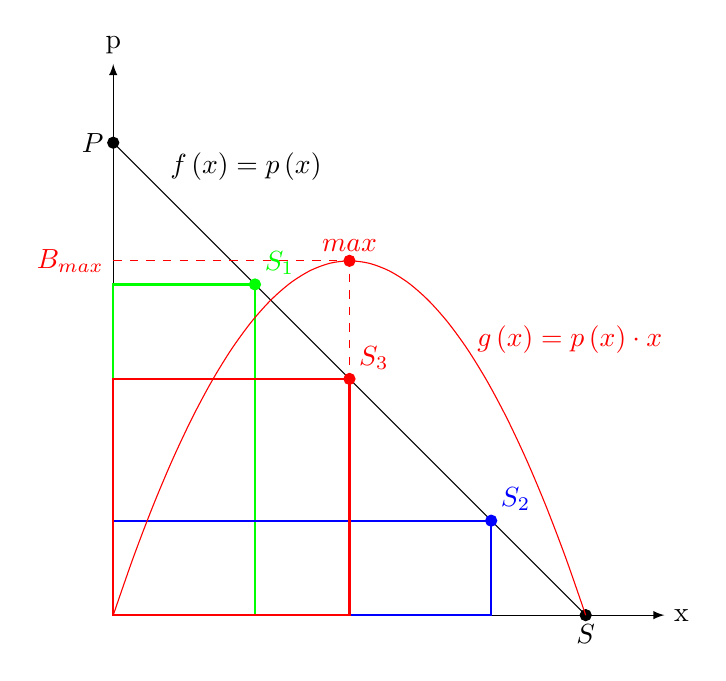
\begin{tikzpicture}
        \draw[->,>=latex,name path=abscissa] (0,0) -- (7,0) node[right] {x};
        \draw[->,>=latex,name path=ordinate] (0,0) -- (0,7) node[above] {p};

        \coordinate (A) at (0,6);
        \coordinate (B) at (6,0);
        \draw[name path=budgetconstraint] (0,6) -- (6,0);

        \filldraw (A) circle (2pt) node[left]  {$P$};
        \filldraw (B) circle (2pt) node[below] {$S$};

        \coordinate (namer) at ($(A)!0.1!(B)$);
        \node[above right] at (namer) {$f\left(x\right)=p\left(x\right)$};

        %% Step 1: S_1 (green, distance 0.3)
        \ifstep{1}{
            \begin{scope}[color=green]
                \coordinate (S1) at ($(A)!0.3!(B)$);
                \filldraw (S1) circle (2pt) node[above right] {$S_{1}$};
                \draw[thick] (0,0) rectangle (S1);
            \end{scope}
        }

        %% Step 2: S_2 (blue, distance 0.8)
        \ifstep{2}{
            \begin{scope}[color=blue]
                \coordinate (S2) at ($(A)!0.8!(B)$);
                \filldraw (S2) circle (2pt) node[above right] {$S_{2}$};
                \draw[thick] (0,0) rectangle (S2);
            \end{scope}
        }

        %% Step 3: S_3 (red, distance 0.5)
        \ifstep{3}{
            \begin{scope}[color=red]
                \coordinate (S3) at ($(A)!0.5!(B)$);
                \filldraw (S3) circle (2pt) node[above right] {$S_{3}$};
                \draw[thick] (0,0) rectangle (S3);
            \end{scope}
        }

        %% Step 4: revenue parabola g(x) with maximum
        \ifstep{4}{
            \begin{scope}[color=red]
                \draw [smooth,domain=0:6] plot ({\x},{-0.5*((\x-3)*(\x-3))+4.5});
                \node[right] at (4.5,3.5) {$g\left(x\right)=p\left(x\right)\cdot x$};
                \coordinate (max) at (3,{-0.5*((3-3)*(3-3))+4.5});
                \filldraw (max) circle (2pt) node[above] {$max$};
                \draw[dashed] (0,|- max) node [left] {$B_{max}$} -- (max) -- (max |-,0);
            \end{scope}
        }

        % \ifstep{2}{
        %     \begin{scope}[color=blue]
        %         \draw[name path=restleft]  (2,0) node[below] {$A_0$} -- (2,7) node[above] {\footnotesize s.t. $A>A_0$};
        %         \draw[name path=restright] (6,0) node[below] {$A_1$} -- (6,7) node[above] {\footnotesize s.t. $A<A_1$};
        %         \draw[name path=redline] plot [smooth,domain=-4:3] ({\x+4},{-2*(0.1*\x^3-0.4*\x^2-0.2*\x+1)+6});
        %         \path [name intersections={of=restleft  and redline,by=leftpoint}];
        %         \filldraw (leftpoint)  circle (2pt) node[below right] {A};
        %         \path [name intersections={of=restright and redline,by=rightpoint}];
        %         \filldraw (rightpoint) circle (2pt) node[below right] {B};
        %         \draw[dashed] (rightpoint) -- (0,|- rightpoint) node[left] {$B_{max}$};
        %     \end{scope}
        % }

    \end{tikzpicture}
\end{document}
